\documentclass{report}
% Change "article" to "report" to get rid of page number on title page
\usepackage{amsmath,amsfonts,amsthm,amssymb}
\usepackage{setspace}
\usepackage{Tabbing}
\usepackage{fancyhdr}
\usepackage{lastpage}
\usepackage{extramarks}
\usepackage{chngpage}
\usepackage{soul,color}
\usepackage{listings}
\usepackage{enumerate}
\usepackage{graphicx,float,wrapfig}
\usepackage{pifont}
\usepackage{graphicx}
\usepackage[english]{babel}
\usepackage{tikz}
\usepackage{algorithm}
\usepackage{algpseudocode}
\usepackage{cite}
% In case you need to adjust margins:
\topmargin=-0.45in      %
\evensidemargin=0in     %
\oddsidemargin=0in      %
\textwidth=6.5in        %
\textheight=9.0in       %
\headsep=0.25in         %

\title{Project - Comp 652 - Machine Learning}

% Homework Specific Information
\newcommand{\hmwkTitle}{Project}                     % Adjust this
\newcommand{\hmwkDueDate}{Thursday, April 23 2015}   % Adjust this
\newcommand{\hmwkClass}{COMP 652}


\newcommand{\hmwkClassInstructor}{Dr. Doina Precup}
\newcommand{\hmwkAuthorName}{Geoffrey Stanley}
\newcommand{\hmwkAuthorNumber}{260645907}
\newcommand{\Pp}{\mathbb{P}}
\newcommand{\Ev}{\mathbb{E}}
\newcommand{\cov}{\text{Cov}}
\newcommand{\Z}{\mathbb{Z}}
\newcommand{\R}{\mathbb{R}}
\newcommand{\dd}{\, \mathrm{d}}

% Setup the header and footer
\pagestyle{fancy}                                                       %
\lhead{\hmwkAuthorName}                              %
\chead{}
\rhead{\hmwkClass: \hmwkTitle}                                          %

\lfoot{}
\cfoot{}                                                                %
\rfoot{Page\ \thepage\ of\ \pageref{LastPage}}                          %
\renewcommand\headrulewidth{0.4pt}                                      %
\renewcommand\footrulewidth{0.4pt}                                      %

% This is used to trace down (pin point) problems
% in latexing a document:
%\tracingall
\definecolor{mygreen}{rgb}{0,0.6,0}
\lstset{commentstyle=\color{mygreen}, frame=single,  language=R, showspaces=false, showstringspaces=false}

%%%%%%%%%%%%%%%%%%%%%%%%%%%%%%%%%%%%%%%%%%%%%%%%%%%%%%%%%%%%%
% Make title
\title{\vspace{2in}\textmd{\textbf{\hmwkClass:\ \hmwkTitle}}\\
\normalsize\vspace{0.1in}\small{Due\ on\ \hmwkDueDate}\\
\vspace{0.1in}\large{\textit{Presented to \hmwkClassInstructor}}\vspace{3in}}
\date{}
\author{\textbf{\hmwkAuthorName}\\
    \textbf{Student ID: \hmwkAuthorNumber}}
%%%%%%%%%%%%%%%%%%%%%%%%%%%%%%%%%%%%%%%%%%%%%%%%%%%%%%%%%%%%%

\begin{document}
\maketitle
\subsection*{Introduction}
The reliability of modern day energy markets is the responsibility of
independent system operators (ISO) who are tasked with the governance of the energy
network within a pre-definied geographic region. PJM Interconnection is such an
organization. It is responsible for the proper functioning of the electric grid
in Delaware, Illinois, Indiana, Kentucky, Maryland, Michigan, New Jersey,
North Carolina, Ohio, Pennsylvania, Tennessee, Virginia, West Virginia and the
District of Columbia.\\

It ensures that loads on the system, such as cities, are
serviced by a sufficient amount of generators, such as nuclear, natural gas or
wind power plants at any given hour of the day. It does so by holding hourly
auctions requesting that producers offer the quantity of megawhatts they are capable of
producing and at what cost. Next, based on the demand for a given hour the ISO
will request that the producers bring their generators online, prioritizing the
most inexpensive power first while also ensuring that the grid operates at a
sufficient level of reliability and redundancy.\\

The first priority of the ISO is the reliability of the system. If it does not
provide a sufficient amount of power to satisfy the loads in the system it
risks causing a brown out or a black out in the entire system. It also must
ensure a certain level of redundancy as if a line or a power plant suddenly
fails the energy grid must continue to operator as a whole. It's second
priority is to provide loads with the most inexpensive power that it can find,
nuclear is cheaper then natural gas, and natural gas cheaper then coal.\\

As such, the price of power through out the energy grid can be seen as being driven
by three categories of variables: demand, supply and physical. With in the demand
component variables will be ones that influence the amount of power being drawn from
the grid. These will be things such as weather, season, day of the week, hour of
the day, weather it's a holiday or normal work week. Supply will be made up of all
factors influencing how generators are changing their bidding behavior. This will
mostly be driven by fuel costs; uranium, natural gas, coal and the amount of wind.
Physical variables will be the current status of the network; what outages and
constraints there are on the system.\\

Congestion in the electricity grid will occur when the price of energy between
two nodes is different. This will occur when different types of generation power
different load zones. For example, take cities A and B both of which consume
100mwh and let's assume that city A is connected to generator E while city B is
connected to F which also produces 200mwh. In a situation where E can produce
200mwh at 15\$ and F at 20\$ there will be no congestion so long as 100mwh
can freely flow between city A and city B. However, if only 50mwh can flow
from A to B then generator F will need to be turned on to produce the remaining
50mwh required by city B. This results in a cost of energy
of 20\$ in city B and a congestion of 5\$ between the two cities.\\

In order to protect generators from unforseen congestion events a product called
up to congestion (UTC) contracts were created. The holder of these contracts will
receive payments when more congestion occurs then expected and have to make payments
when less congestion the expected occurs.\\

Which creates the problem of how to accurately evaluate the value of these contracts.\\

\subsection*{Methodology}
Ignoring potential variables such as fuel costs, weather and outages; as a first
attempt in trying to evaluate the value of a UTC contract a Markov
Chain Monte Carlo (MCMC) approach will be used. The objective will be to use the
previous distribution of differences between UTC contract prices and the last
known price to estimate the most likely value in the future. A similar method to
the one used by Landauskas \cite{landauskas} to evaluate future stock prices will
be used.\\

The first step will be the estimation of the distribution for price differences
for a particular time range. This will be done using SciPy's \cite{scipy}
implementation of Gaussian kernel density estimate (KDE). This implementation will
also allow for the generation of a set of random samples from the distribution.
Once the random samples are generated, they will be added to the previous known
price of the contract and the Gaussian KDE will again be used to infer the
distribution of potential future contract prices. The price with the greatest
likelihood will be used as the forecasted price. The evaluation of the model's accuracy will
be done by summing the squared error of the differences between the forecasted prices
and the actual prices.\\

Due to the seasonality of the prices the amount of history used to estimate the
probability distribution of price differences will need to be optimized. As such,
a time series validation procedure will need to be used. This procedure will be
implemented as follows: at $t_0$ the price at $t_1$ will be predicted using price
difference distributions between $t_{0-n} \rightarrow t_0$ where $n$ will vary in days
between one week and one year.\\

In order to attempt to reduce the effect of variables outside of normal seasonality
aggregates of nodes were selected; Eastern Hub and Western Hub. These hubs are an average
of a few hundred different pricing nodes within their regions.\\

Price differences between Eastern Hub and Western Hub from
January first 2013 and January first 2015 can be seen in the following figure:

\begin{center}
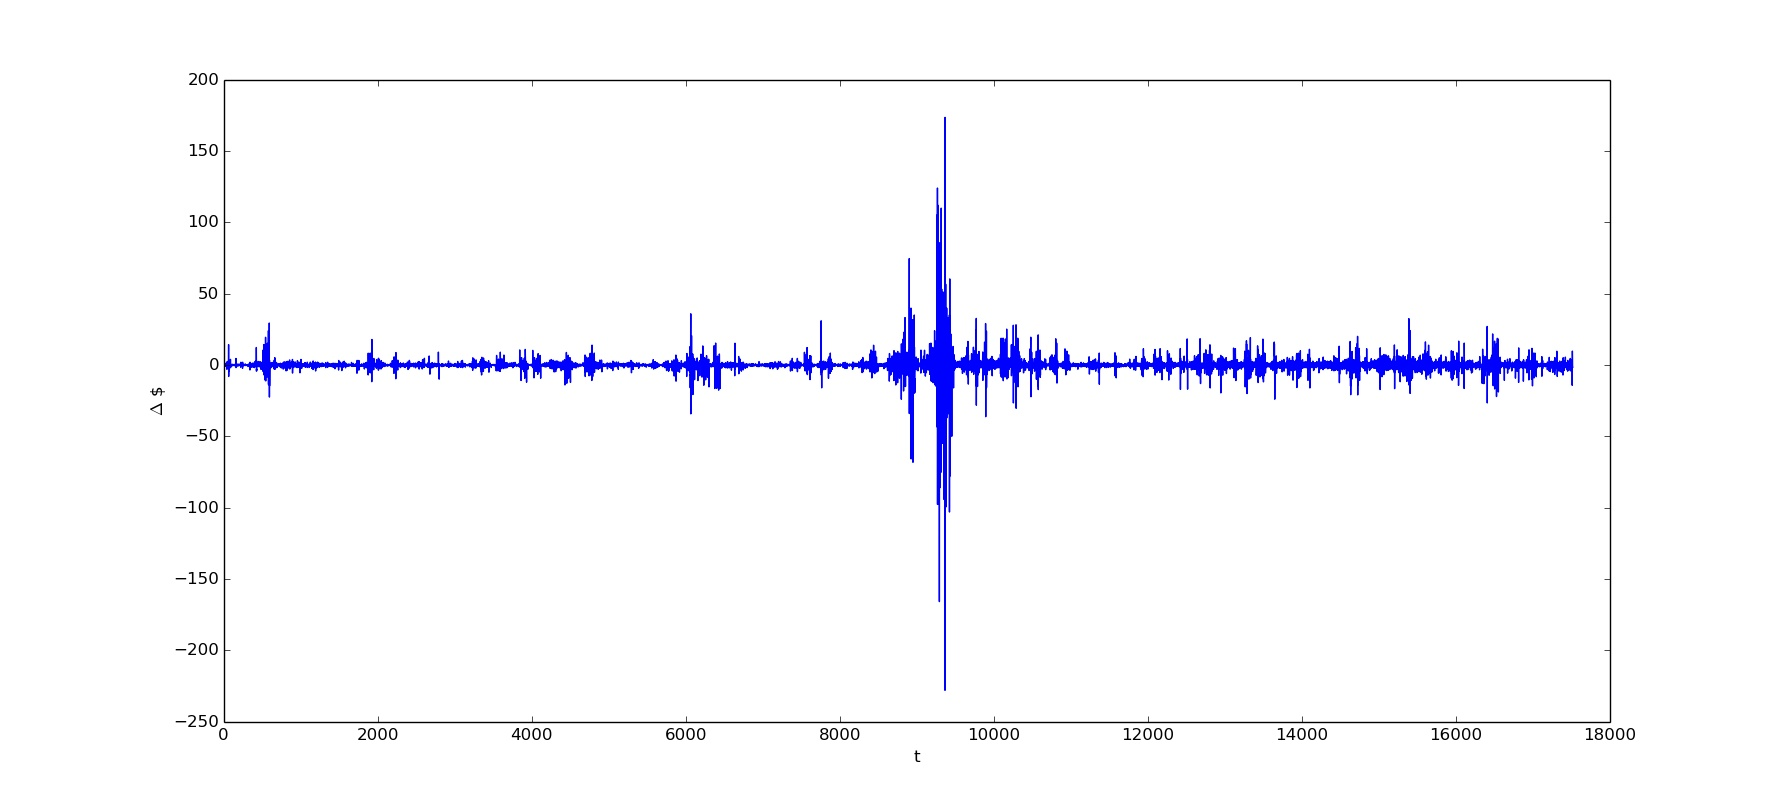
\includegraphics[width=500pt, keepaspectratio=true]{price_differences.jpg}
\end{center}

Differences were consistent except for a period in January 2014. Because of the
tendency of the differences to be within a rather tight range the next optimization
problem will be deciding how many of the outliers to remove when evaluating the
data distribution.\\

As a second step, after the optimal amount of history to be used is identified, the
same use the same process described previously for forecasting a ptice at $t_1$
however in this approach the amount of outliers removed will vary. From the bottom
and top $0\%$ to $25\%$.\\

Lastly, the differences in price distributions between hours of the day is significant:
\begin{center}
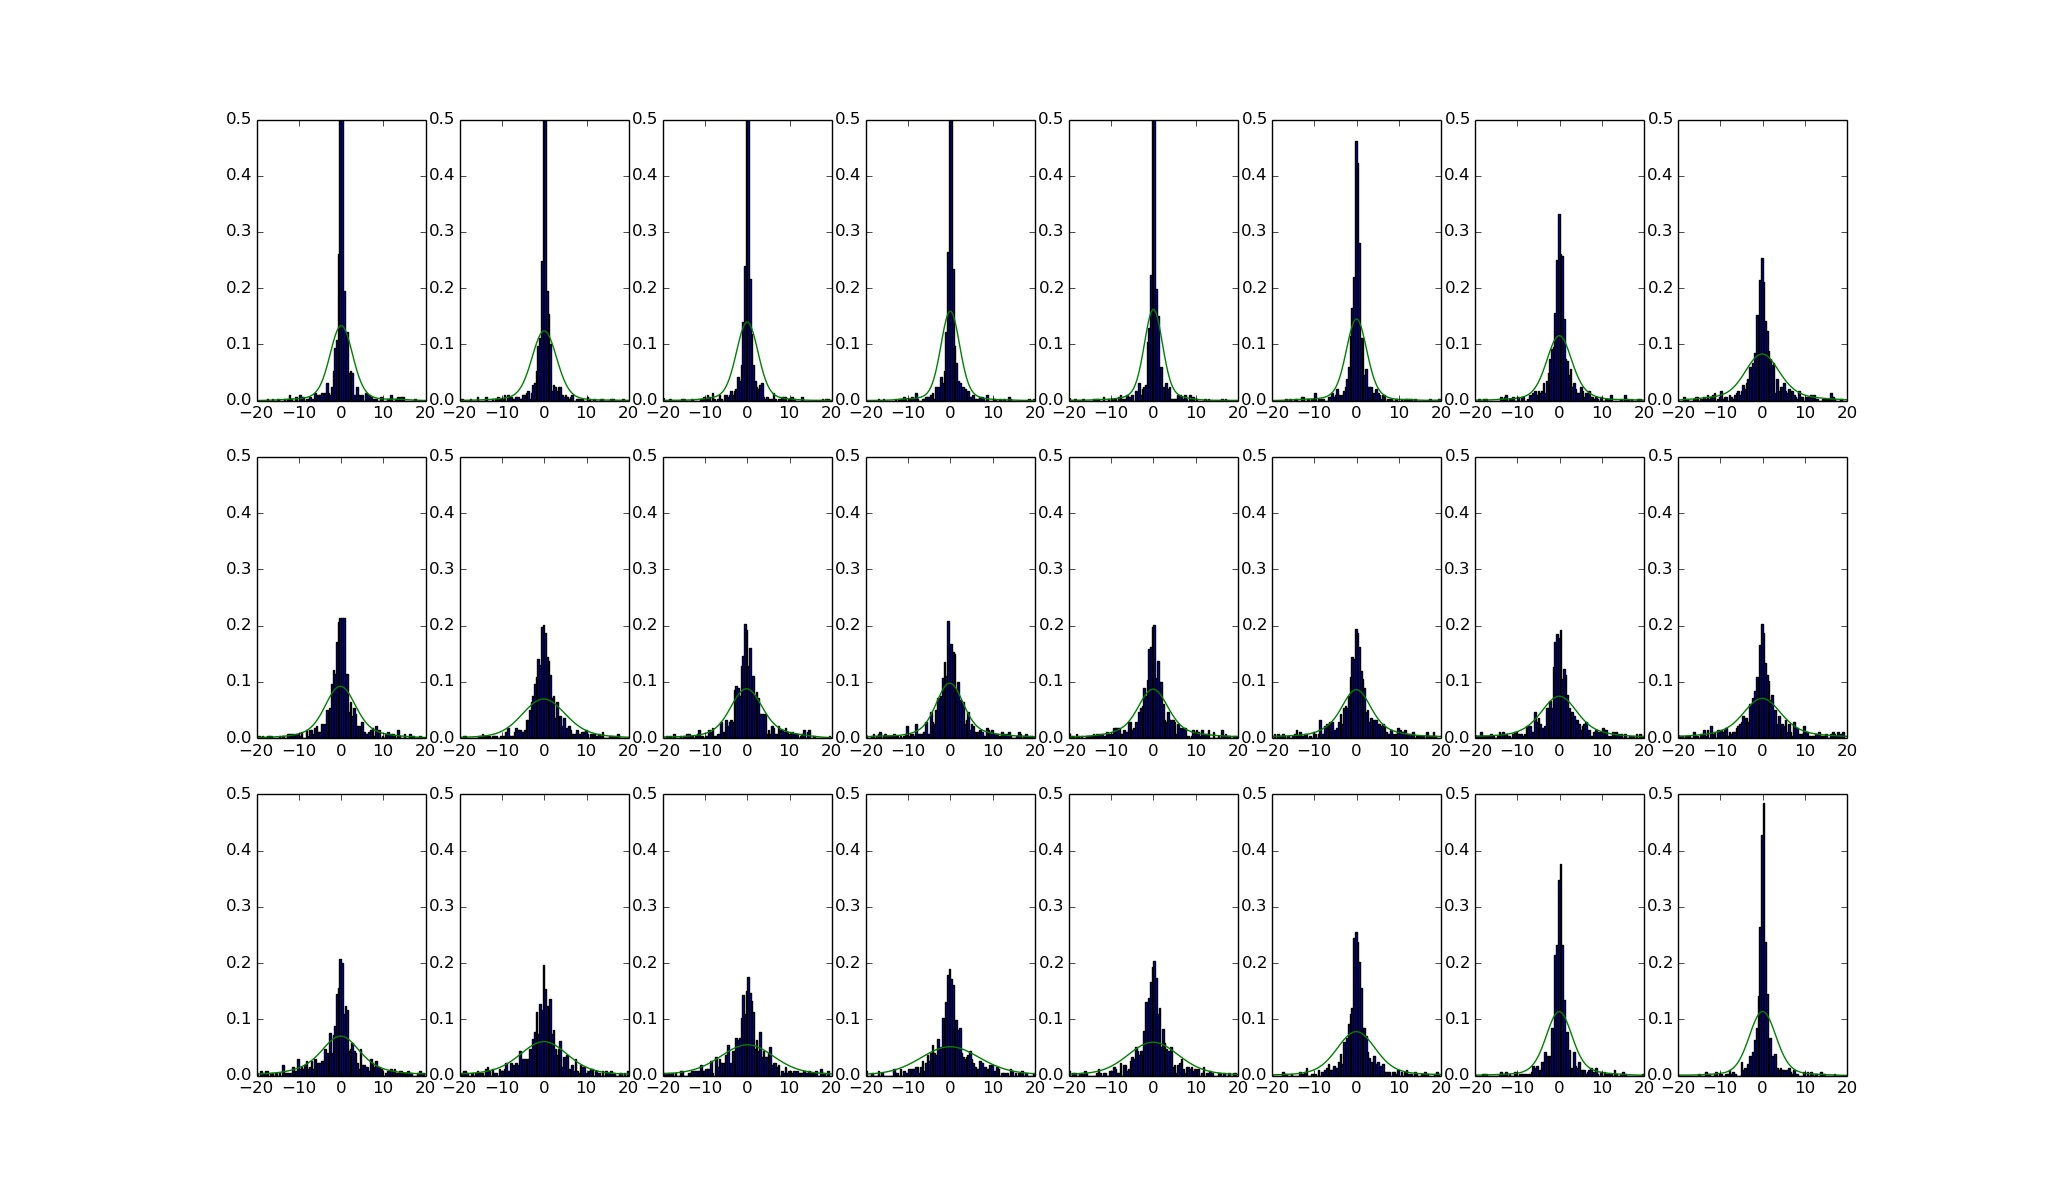
\includegraphics[width=500pt, keepaspectratio=true]{hourly_distributions.jpg}
\end{center}
The figure above shows the price differences for hours ending 0 through 23. The x-axis
is the difference in price and the y-axis is the probability 0 to 1 of that difference.
Evening hours 22, 23 and 0 through 6 are much less volatile then the others. As such,
the UTC contracts should be evaluated on an hourly basis given the price it was
worth at the same hour the previous day.

\subsection*{Experimental Set-up}
Data was obtained from the PJM website \cite{pjm}. Data was extracted using their
eData service. Specifically, data for the Eastern Hub and Western Hub nodes between
January 1st 2013 and January 1st 2015. Two database tables were created for each
of the nodes and the were subsequently joined by timestamp in order to be able to
calculate congestion between the two nodes. Congestion beeing the price of the
energy component in the Eastern Hub minus the price of the energy components in the
Western Hub.

Once this data was generated the data was further split into 24 tables for the 24 hours
of the day. With these tables I was able to calculate the difference in price from
one day to the next for a particular hour.



\subsection*{Results}
The following figure shows the means squared error produced by the model as a
function of the amount of history used to fit the model.

\begin{center}
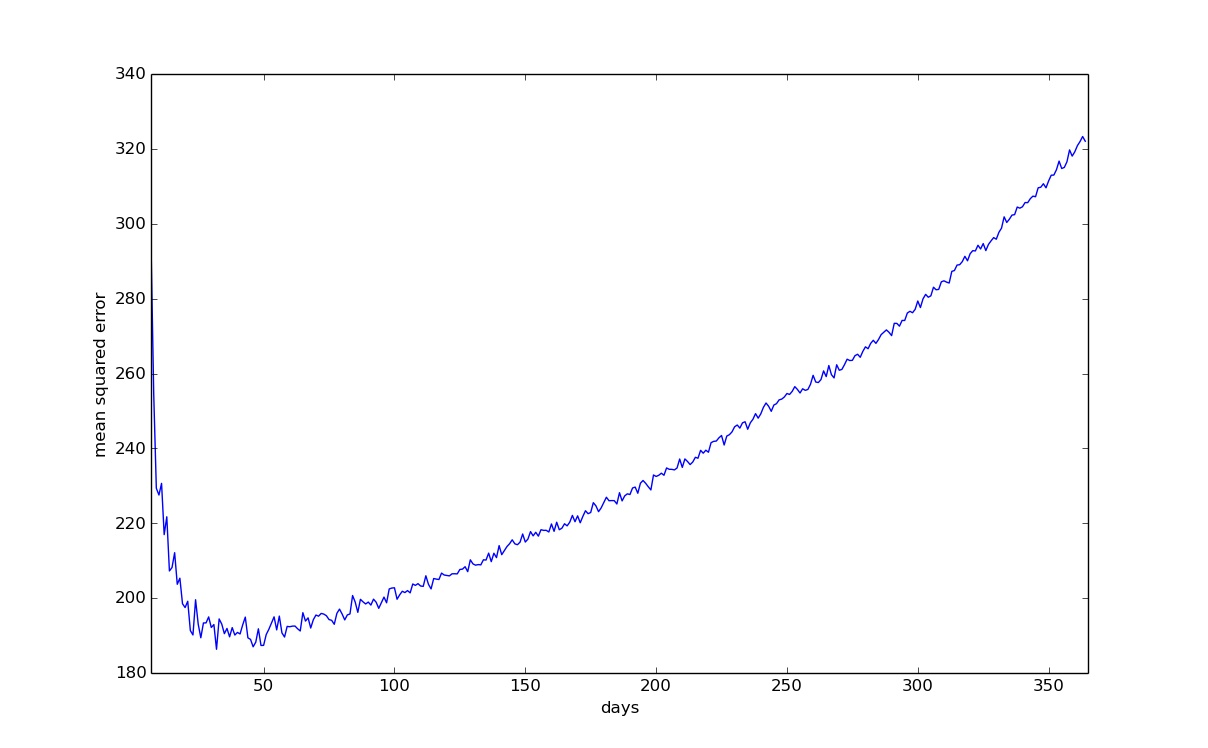
\includegraphics[width=250pt, keepaspectratio=true]{mean_squared_error.jpg}
\end{center}

This shows that the optimum amount of history to be used is about 30 days.

The next figure shows the improvement of mean squared error as outliers are removed:
\begin{center}
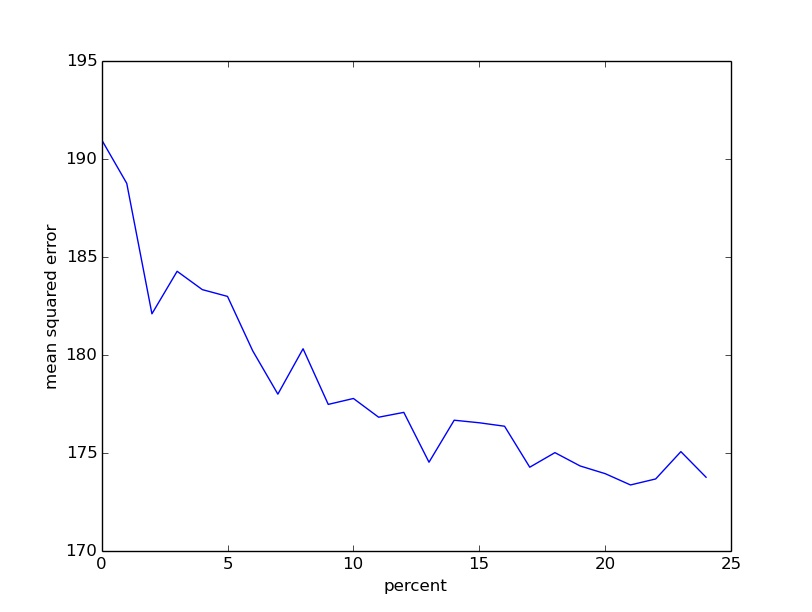
\includegraphics[width=250pt, keepaspectratio=true]{outlier_error.jpg}
\end{center}
The interpretation of this graph leads me to believe that predictive feature for
future prices is no the distribution of price differences but in fact the actual
price at $t_{0-1}$. This is because accuracy continues to increase as fewer and
fewer data points are used to evaluate the price difference distribution. I believe
this is caused by the mean reverting nature of the price of the contracts.

\subsection*{Conclusions}

One of the weaknesses of this approach is that it does not take into account the
mean reverting tendency of energy prices. In other words, when a price suddenly
jumps this approach to modelizing the price behavior assumes that the price will
maintain the price it moved to. A more robust approach would need to take into account
how strong the tendency is to revert to a mean price and what that mean is.\\

Further work would also need to take into account more of the features. One potential
avenue would be to look at price differences given particular outages in the system.
As well as incorporate supply and demand drivers such as fuel costs and weather.

\nocite{*}
\bibliography{bibliography}
\bibliographystyle{plain}

\end{document}
